\documentclass{article}

% PACKAGES  ****************************************************************
\usepackage{lipsum}		% Used to generate dummy-text (\lipsum[1])
\usepackage[margin=2.54cm,includefoot]{geometry}		% Used to control margins

\usepackage{graphicx} % allows to import images
\usepackage{float}	% allows for control of float positions
\usepackage{tikz} 	% Used to create trees
\usepackage[hidelinks]{hyperref}	% allows for clickable references

\usepackage[numbers,sort&compress]{natbib} 	% sorts the cites in increasing order automatically when referenced and compresses successive references

\usepackage[english,german]{babel}		% Change language from english to german (order matters!)

\usepackage{fancyhdr}	% Used for Header and Footer stuff

\usepackage{xfrac}	% allows for slanted fractions 
% ****************************************************************

% HEADER AND FOOTER STUFF ****************************************************************
\pagestyle{fancy}
\fancyhead{}	% clears header
\fancyfoot{}	% clears footer
\fancyfoot[R]{\thepage}	% sets position right
\renewcommand{\headrulewidth}{0pt}	% removes header line by setting it to zero
\renewcommand{\footrulewidth}{1pt}		% add footer line by setting it to one
% ****************************************************************

% DEFINE LIST ITEM BULLETS ****************************************************************
\renewcommand{\labelitemi}{$\bullet$}	% first list item
\renewcommand{\labelitemii}{$\circ$}	% one-indented item
\renewcommand{\labelitemiii}{$\diamond$}	% twice-indented item
% ****************************************************************


\begin{document}

% TITLE PAGE ****************************************************************
\begin{titlepage}
	
	\begin{center}
	\line(1,0){330} \\
	[2mm]
	\huge{\bfseries Data Science Zusammenfassung} \\
	[2mm]
	\line(1,0){320} \\
	[1,5cm]
	\textsc{\LARGE By Yannis Schmutz} \\
	[0.75cm]
	\textsc{\large todo} \\
	
	\end{center}
	
\end{titlepage}
% ****************************************************************

% PREFACE STUFF ****************************************************************
\pagenumbering{roman}		% sets the page numbering to roman for the preface etc.
\section*{Zusammenfassung}	% Adds a section without a number in front
\addcontentsline{toc}{section}{\numberline{}Zusammenfassung}	% adds a section without a number in front to the ToC
\cleardoublepage	% Finishes the current page so that the following page will always be odd.
% ****************************************************************

% TABLE OF CONTENTS ****************************************************************
\renewcommand{\contentsname}{Inhaltsverzeichnis}	% Rename table of contents to the german version
\tableofcontents		% adds table of contents (this needs to be compiled twice sometimes in order to update)
\thispagestyle{empty}	% removes header & footer on this page
\cleardoublepage	% Finishes the current page so that the following page will always be odd.
% ****************************************************************

% LIST OF FIGURES ****************************************************************
%\renewcommand{\listfigurename}{Abbildungsverzeichnis}	% renames list of figures
\listoffigures	% generates a list of figures
\addcontentsline{toc}{section}{Abbildungsverzeichnis}	% Adds list of figures to the ToC
\cleardoublepage
% ****************************************************************

% LIST OF TABLES ****************************************************************
%\renewcommand{\listtablename}{Tabellenverzeichnis}
\listoftables
\addcontentsline{toc}{section}{Tabellenverzeichnis}
\cleardoublepage
% ****************************************************************

% START OF REGULAR CHAPTERS ****************************************************************
\setcounter{page}{1}		% Sets this page to the first one (and not the table of contents)
\pagenumbering{arabic}	% Sets the page numbering back to arabic
% ****************************************************************

% ****************************************************************
\section{Einleitung}\label{sec:intro}
\lipsum[1]
% ****************************************************************

% ****************************************************************
\newpage
\section{Statistik}\label{sec:stat}
\lipsum[1]
% ****************************************************************

% ****************************************************************
\newpage
\section{Probabilistik}
\subsection{Bedingte Wahrscheinlichkeit}

\subsubsection{Satz von Bayes}
Verweis auf Kapitel \pageref{sec:stat}.
% ****************************************************************



% TRYOUT PART ****************************************************************
\newpage
\section{Tryout}\label{sec:tryout}

\begin{figure}[H]	% H stands for here (place right here)
	\centering
	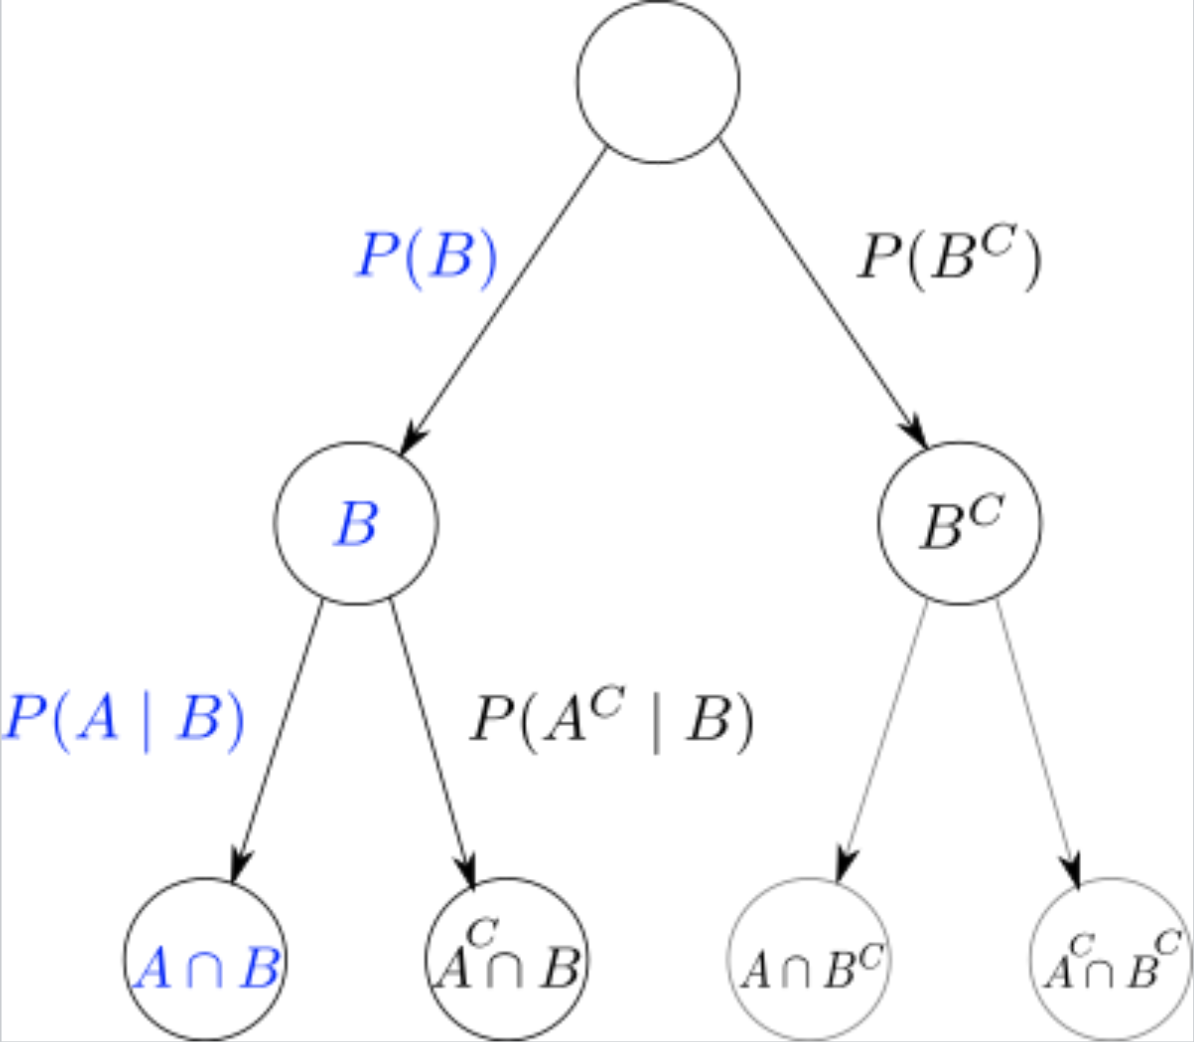
\includegraphics[height=5cm]{figures/tryout.png}
	\caption[Optional optional]{Entscheidungsbaum}
	\label{fig:tryout}
\end{figure}

Wie auf der Abbildung \ref{fig:tryout} zu sehen ist.....


\begin{table}[H]
	\centering
	\label{tab:tryouttab}
\caption[This is an optional caption, without reference]{Local caption, with reference}
	\cite{ref:ds_1, ref:nn_1, ref:ai_1}	% Used to add cites (zitieren)

	\begin{tabular}{l c r}
		Area & Number of rooms & Price \\ \hline
		80	& 4				& 1680 \\
		100	& 5				& 2300 \\
		50	& 2.5				& 1500 \\
		
	\end{tabular}
\end{table}


\begin{itemize}
	\item This is an item
	\item This is another item
	\begin{itemize}
		\item This is a further item
		\item [blub] This is an item with a custom bullet point
	\end{itemize}
\end{itemize}

\begin{enumerate}
	\item This is a numbered item
	\item And so on
\end{enumerate}


\newpage
\subsection{Math examples}

Here's an example within a sentence $E =mc^2$.

And here one example $$a=v/t$$ which is centred. \\

$$-\frac{\hbar^2}{2m}\frac{d^2\Psi}{dx^2} = E\Psi$$

Fractions

$$d = v_it + \frac{1}{2} \cdot at^2$$
$$d = v_it + \sfrac{1}{2} \cdot at^2$$


Brackets:
$$\left( \frac{1}{2} \right) \cdot 2 = 1$$	% use \left( ..... \right) to match the brackets to the content
$$\left| -7 \right| = 7$$
$$\sqrt{4} = 2$$
$$\sqrt{4} \ne 1$$
$$\sqrt{4} < 5$$
$$ \pi \approx 3 $$
$$ \pi \times \sqrt{4} < 15 $$

\begin{eqnarray}	% Equation array
	3x + 14 &=& 20 \\
	3x &=& 6 \\
	x &=& 2
\end{eqnarray}

\begin{equation}
\label{eq:first}
x^2 + 3x - 7 = 0
\end{equation}

\newpage
\subsection{Graphs}

\begin{tikzpicture}[every node/.style={circle, draw=black}]
	[align=center, sibling distance=5cm]
	\node[fill=black]{}
		child { node{B} 
			child { node{A $\cap$ B} }
			child { node{$\bar{A} \cap B$} }
			}
		child{ node{$\bar{B}$} 
			%child{ node{$A \cap \bar{B}$} }
			child{ node{$\bar{A} \cap \bar{B}$} }
		       }
	;

\end{tikzpicture}
% ****************************************************************


% REFERENCES ****************************************************************
\cleardoublepage
%\renewcommand{\bibname}{Referenzen}	% Rename the bibliography title
\bibliographystyle{IEEEtran}	% Adds cites (Zitate)
\addcontentsline{toc}{section}{Referenzen}
% references can easily be generated using the OS X tool "BibDesk"
% Make sure you build your LaTeX document in BibTeX after defining your references
%	in order to make them valid.
\bibliography{references/book_ref1.bib}
% ****************************************************************

% APPENDIX ****************************************************************
\cleardoublepage
\appendix
\section{Cheatsheet}
% ****************************************************************


\end{document}